\documentclass[8pt]{beamer}
\usepackage[utf8x]{inputenc} % Включаем поддержку UTF8  
\usepackage[T2A]{fontenc}
\usepackage[english,russian]{babel}  % Включаем пакет для поддержки русского языка 
\usepackage{graphicx}
\graphicspath{{pictures/}}
\usetheme{JuanLesPins}
\usecolortheme{beaver}

%\usepackage{fontspec}
%\defaultfontfeatures{Ligature={Tex}, Renderer=Basic}
%\setmainfont[Ligatures={Tex, Historic}]{georgia}

%\usepackage[fontsize=8]{scrextend}
%\setbeamerfont{title}{family=\rmfamily}

\usepackage{lmodern}
\usepackage{fix-cm}
\usepackage{kurier}

\title {Broken RSA}
\author {Подготовили: Воробьёв Д.	Нецветайлов А., КБ-2}
\institute{Балтийский Федеральный университет им. Иманнуила Канта, Калининград}
\date[1 июля 2022]{1 июля 2022}

\begin{document}
\frame[plain]{\titlepage}	


\begin{frame}
	\begin{block}
	{
		\frametitle{Квадратичный вычет \\ Символ Лежандра}
		\textbf{Квадратичныый вычетом} по модулю $m$ называется такое целое число $a$, для которого выполняется тождество
	
		$x^2 \equiv \pmod m$
	
		Если сравнение не разрешимо, то число $a$ называют квадратичным \textbf{невычетом}}
	\end{block}
	
	\begin{block}
	{
		\textbf{Символ Лежандра} — функция, используемая в теории чисел. Введён французским математиком А. М. Лежандром.
	
		Пусть $a$ - целое число и $p$ - просто число, отличное от $2$ Символ Лежандра $\frac{a}{p}$ определяется следующем образом:
		\begin{itemize}
		\item $\frac{a}{p} = 0$, если $a$ делится на $p$;
	
		\item $\frac{a}{p} = 1$, если $a$ является квадратичным вычетом по модулю $p$, но при этом $a$ не делится на $p$;
	
		\item $\frac{a}{p} = -1$, если $a$ является квадратичным невычетом по модулю $p$.
		\end{itemize}
	}
	\end{block}
\end{frame}


\begin{frame}
	\frametitle{Алгоритм Тонелли-Шенкса}
	%\begin{figure}
	%	\includegraphics[scale=0.16]{Tonelli-Shenks Algorithm.png}
	%\end{figure}
	\textbf{Входные данные:} $p$ — нечётное простое число, $n$ — целое число, являющееся квадратичным вычетом по модулю $p$, другими словами, $n/p = 1$, где $ab$ — символ Лежандра. 
	$x^2 ≡ n \pmod p$
	
	\textbf{Результат работы алгоритма:} вычет $R$, удовлетваряющий сравнению $R^2\equiv n\pmod p$
		
		\textbf{1.} Выделим степени двойки из $p-1$, то есть пусть $p-1=2^SQ$ где $Q$ нечётно, $S >= 1$. Заметим, что если S=1, то есть $p\equiv3\pmod4$, тогда решение определяется формулой $R\equiv \pm n^ \frac{p+1}{4}$. Далее полагаем $S>=2$
		
		\textbf{2.} Выберем произвольный квадратичный вычет $z$, то есть символ Лежандра $\frac{z}{p} = -1$, положим $c\equiv z^Q \pmod p$
		
		\textbf{3.} Пусть также $R \equiv n \frac{Q+1}{2} \pmod p$, $t \equiv n^Q \pmod p$, $M=S$
		
		\textbf{4.} Выполняем цикл:
		
		\begin{itemize}
			\item Если $t \equiv 1 \pmod p$, то алгоритм возвращает R
		
			\item В проивном случае в цикле находим наименьшее $i$, $0 <i<M$, такое, что $(t^2)^i \equiv 1 \pmod p$ с помощью итерирования возведения в квадрат.
		
			\item Пусть $b \equiv (c^2)^(M-i-1) \pmod p$, и положим $R: \equiv Rb \pmod p$, $t: \equiv tb^2 \pmod p$, $c \equiv b^2 \pmod p$, $M := i$, возвращаемся к началу цикла
		\end{itemize}
	
	После нахождения решения сравнения $R$ второе рещение сравнение находится как $p-R$
\end{frame}


\begin{frame}
	\frametitle{Задача}
	
	\begin{figure}
		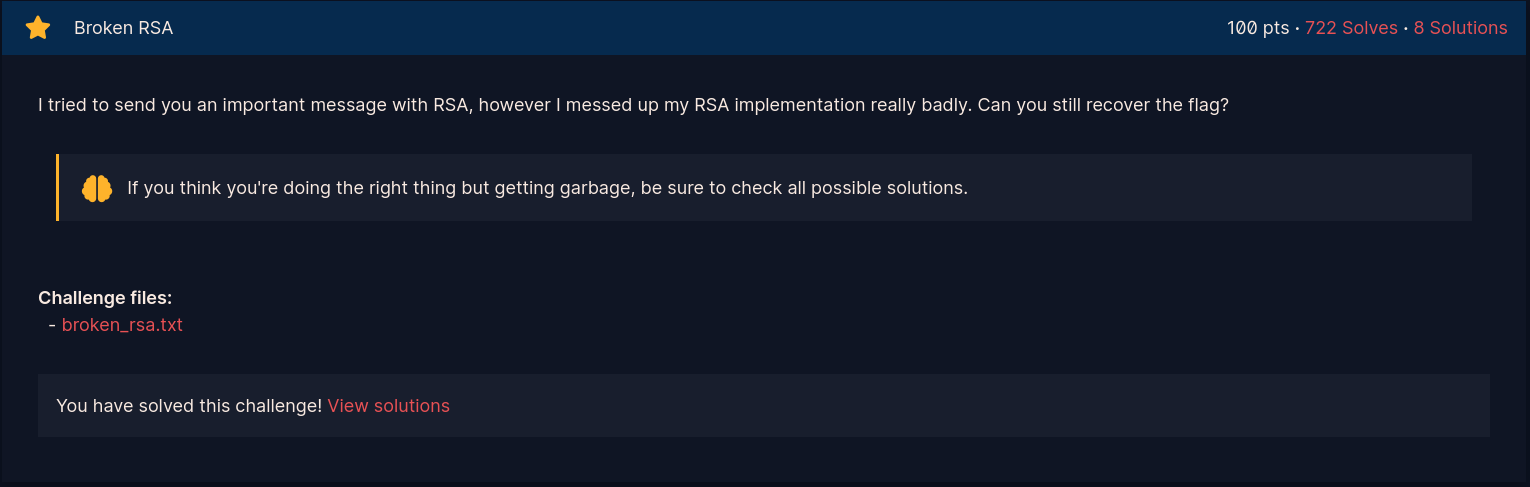
\includegraphics[scale=0.2]{Brocken RSA.png}	
	\end{figure}
		
\end{frame}

\end{document}
